\chapter{Конструкторская часть}

% =====================================================
\section{Функциональная модель программного обеспечения}

На рисунке \ref{img:idef0_func} представлена функциональная модель программного обеспечения.

\begin{figure}[h]
	\begin{center}
		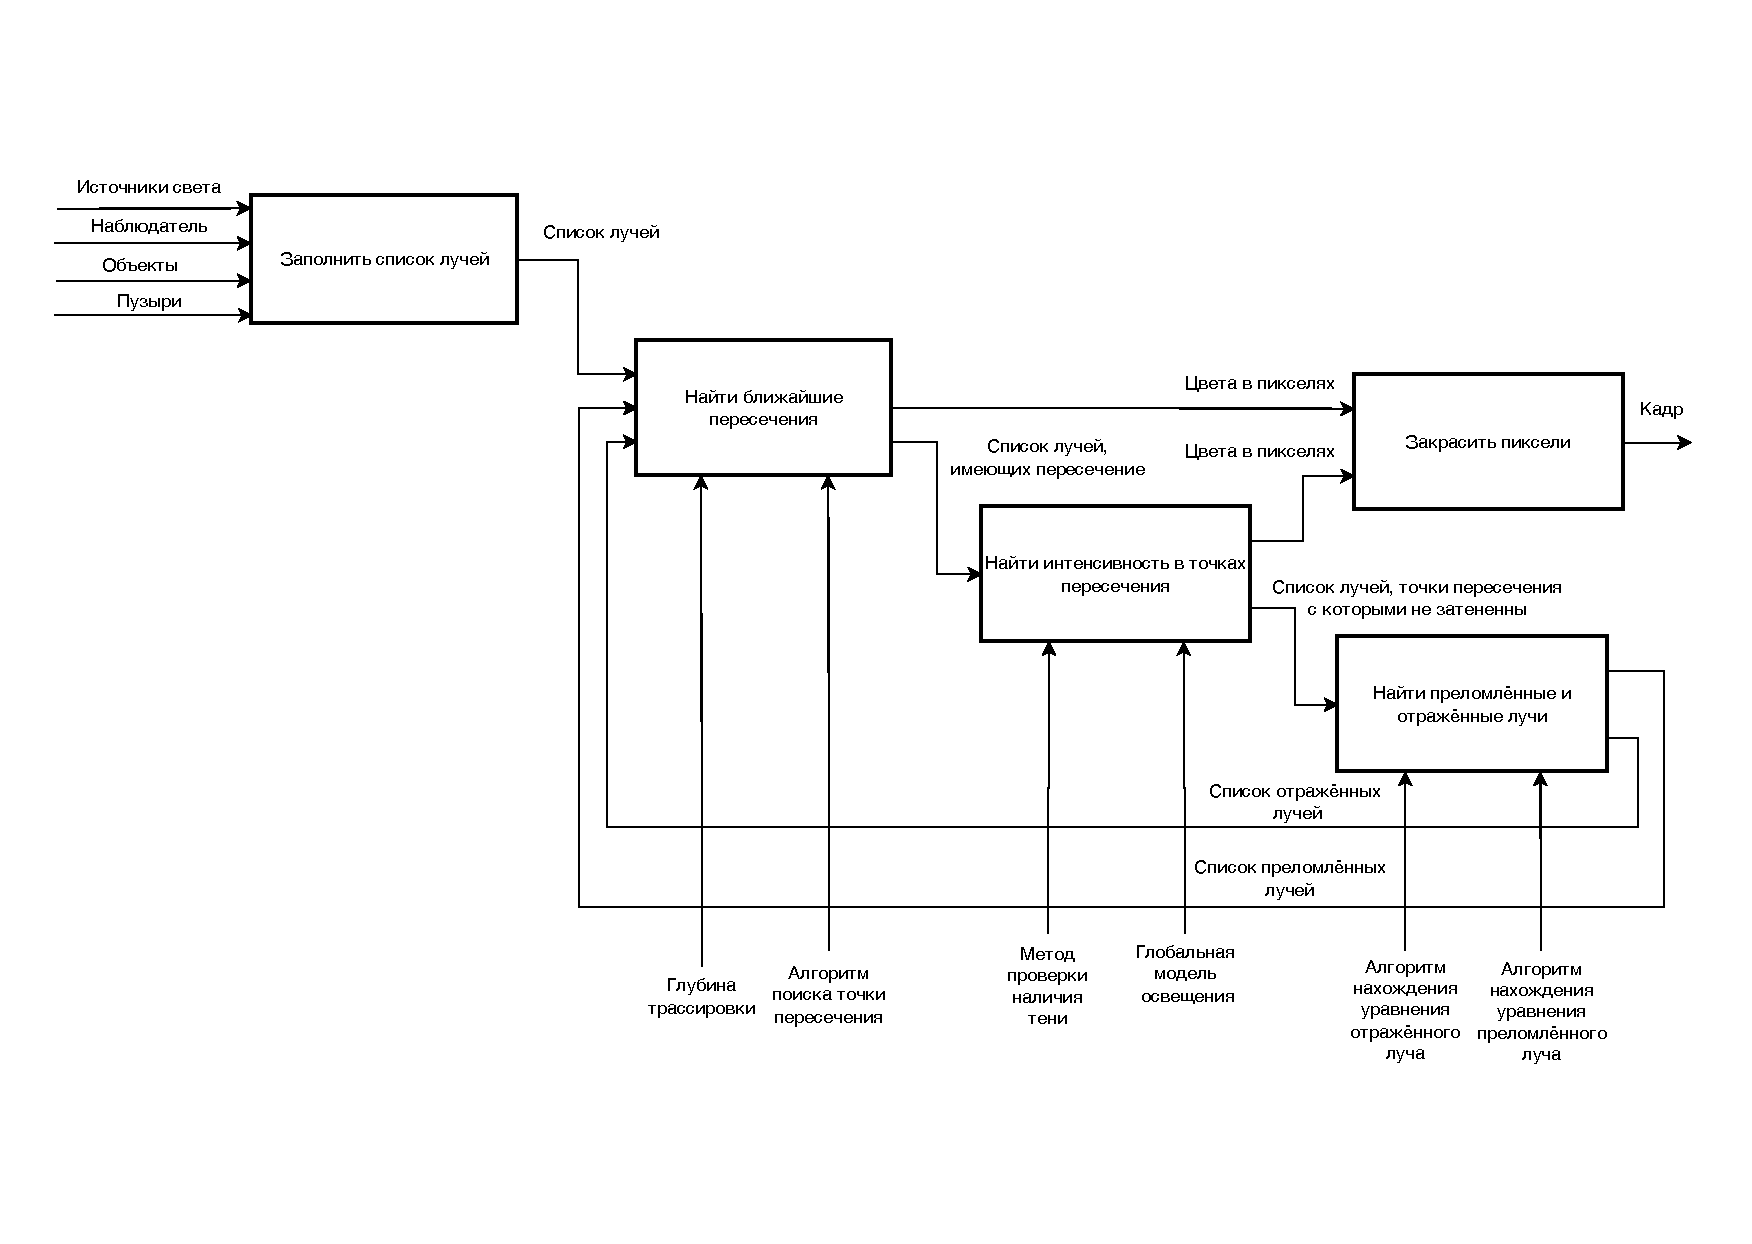
\includegraphics[width=\linewidth]{img/idef0_func.pdf}
	\end{center}
	\captionsetup{justification=centering}
	\caption{Функциональная модель программного обеспечения}
	\label{img:idef0_func}
\end{figure}


\clearpage

% =====================================================
\section{Используемые типы и структуры данных}

В данном пункте описываются типы и структуры данных, используемые в программном обеспечении.

\begin{enumerate}[label={\arabic*)}]
	\item Сцена, состоящая из:
    \begin{itemize}[label=---]
		\item массива объектов;
		\item наблюдателя;
		\item массива источников света.
	\end{itemize}

	\item Объект, состоящий из материала.
 
	\item Триангулированный объект, состоящи из: 
    \begin{itemize}[label=---]
		\item массива вершин (координаты типа вектор);
		\item массива полигонов.
	\end{itemize}
 
	\item Полигон, являющийся массивом из трёх указателей на вершины.
 
	\item Сфера, состоящая из
    \begin{itemize}[label=---]
		\item центра (координаты типа вектор);
		\item радиуса (положительное вещественное число).
	\end{itemize}

    \item Пузырь, состоящий из
    \begin{itemize}[label=---]
		\item внешнего слоя (сфера);
        \item внутреннего слоя (сфера).
	\end{itemize}
 
	\item Источник света, состоящий из:
    \begin{itemize}[label=---]
		\item расположения (координаты типа вектор);
		\item интенсивности (вещественное число от 0 до 1).
	\end{itemize}
 
	\item Камера, состоящая из:
    \begin{itemize}[label=---]
		\item расположения (координаты типа вектор);
		\item направления взгляда (координаты типа вектор)
	\end{itemize}
 
	\item Материал, состоящий из:
    \begin{itemize}[label=---]
		\item цвета объекта (три целочисленных переменных в модели $RGB$);
		\item коэффициента фонового освещения (вещественное число от 0 до 1);
		\item коэффициента диффузного освещения (вещественное число от 0 до 1);
		\item коэффициента зеркального освещения (вещественное число от 0 до 1);
		\item дисперсия (вещественное неотрицательное число);
		\item коэффициента преломления (вещественное неотрицательное число);
        \item показателя отражения (вещественное неотрицательное число);
		\item показатель преломления (вещественное неотрицательное число).
	\end{itemize}
\end{enumerate}

% =====================================================
\section{Формальное описание алгоритмов}

Основные алгоритмы, используемые в программном обеспечении вынесены в схемы, представленные на рисунках \ref{img:trace_ray}-\ref{img:tr_intersection_2}.

\begin{figure}[H]
	\begin{center}
		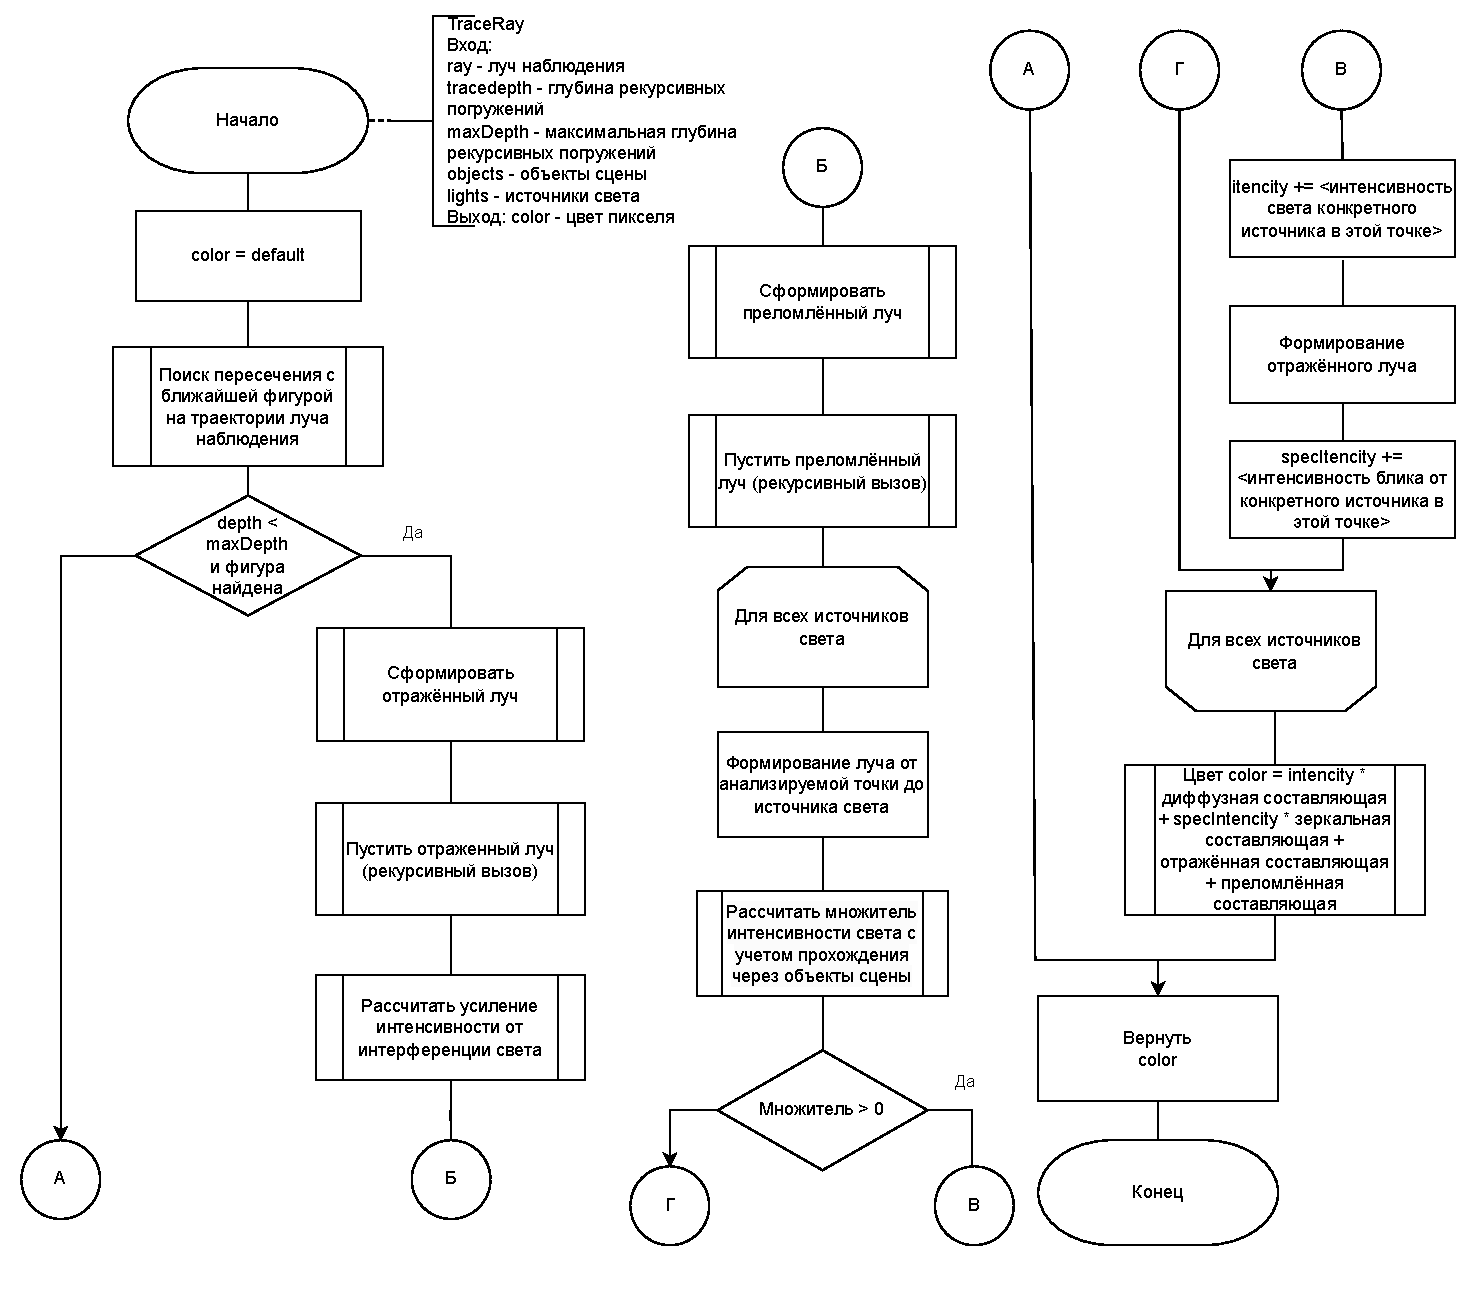
\includegraphics[width=\linewidth]{img/trace_ray.pdf}
	\end{center}
	\captionsetup{justification=centering}
	\caption{Схема алгоритма трассировки лучей}
	\label{img:trace_ray}
\end{figure}

\begin{figure}[H]
	\begin{center}
		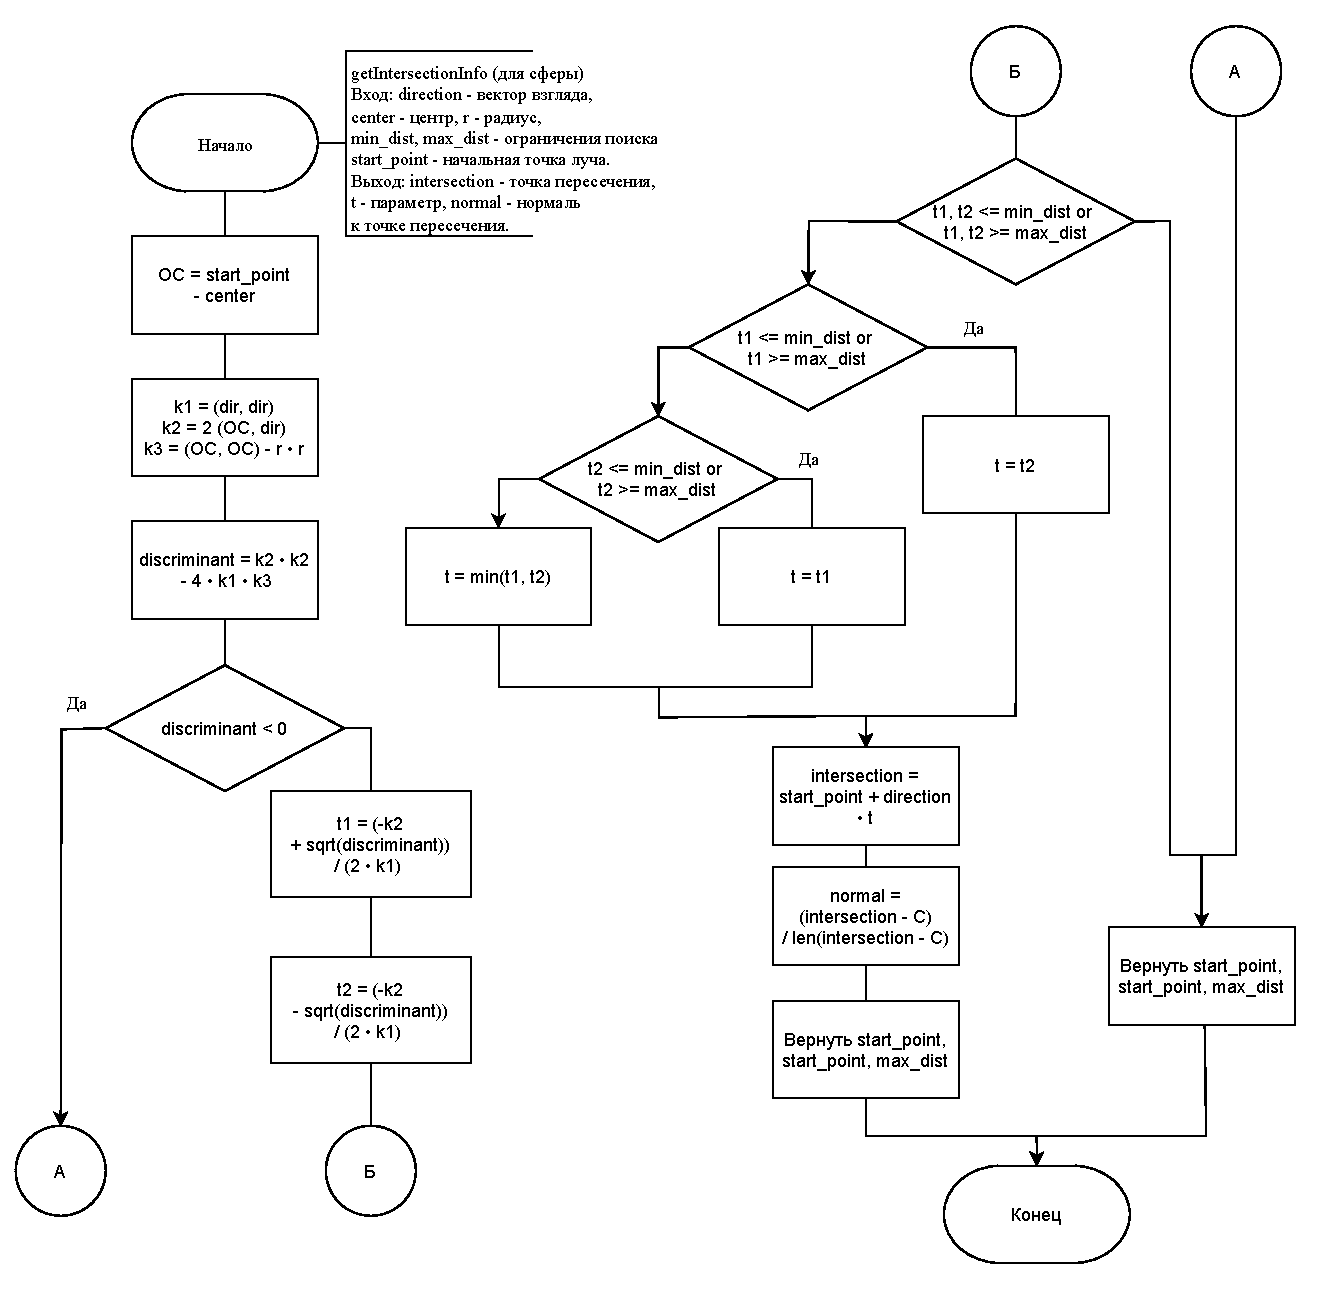
\includegraphics[width=\linewidth]{img/sphere_intersection.pdf}
	\end{center}
	\captionsetup{justification=centering}
	\caption{Схема алгоритма поиска пересечения луча со сферой}
	\label{img:sphere_intersection}
\end{figure}

\begin{figure}[H]
	\begin{center}
		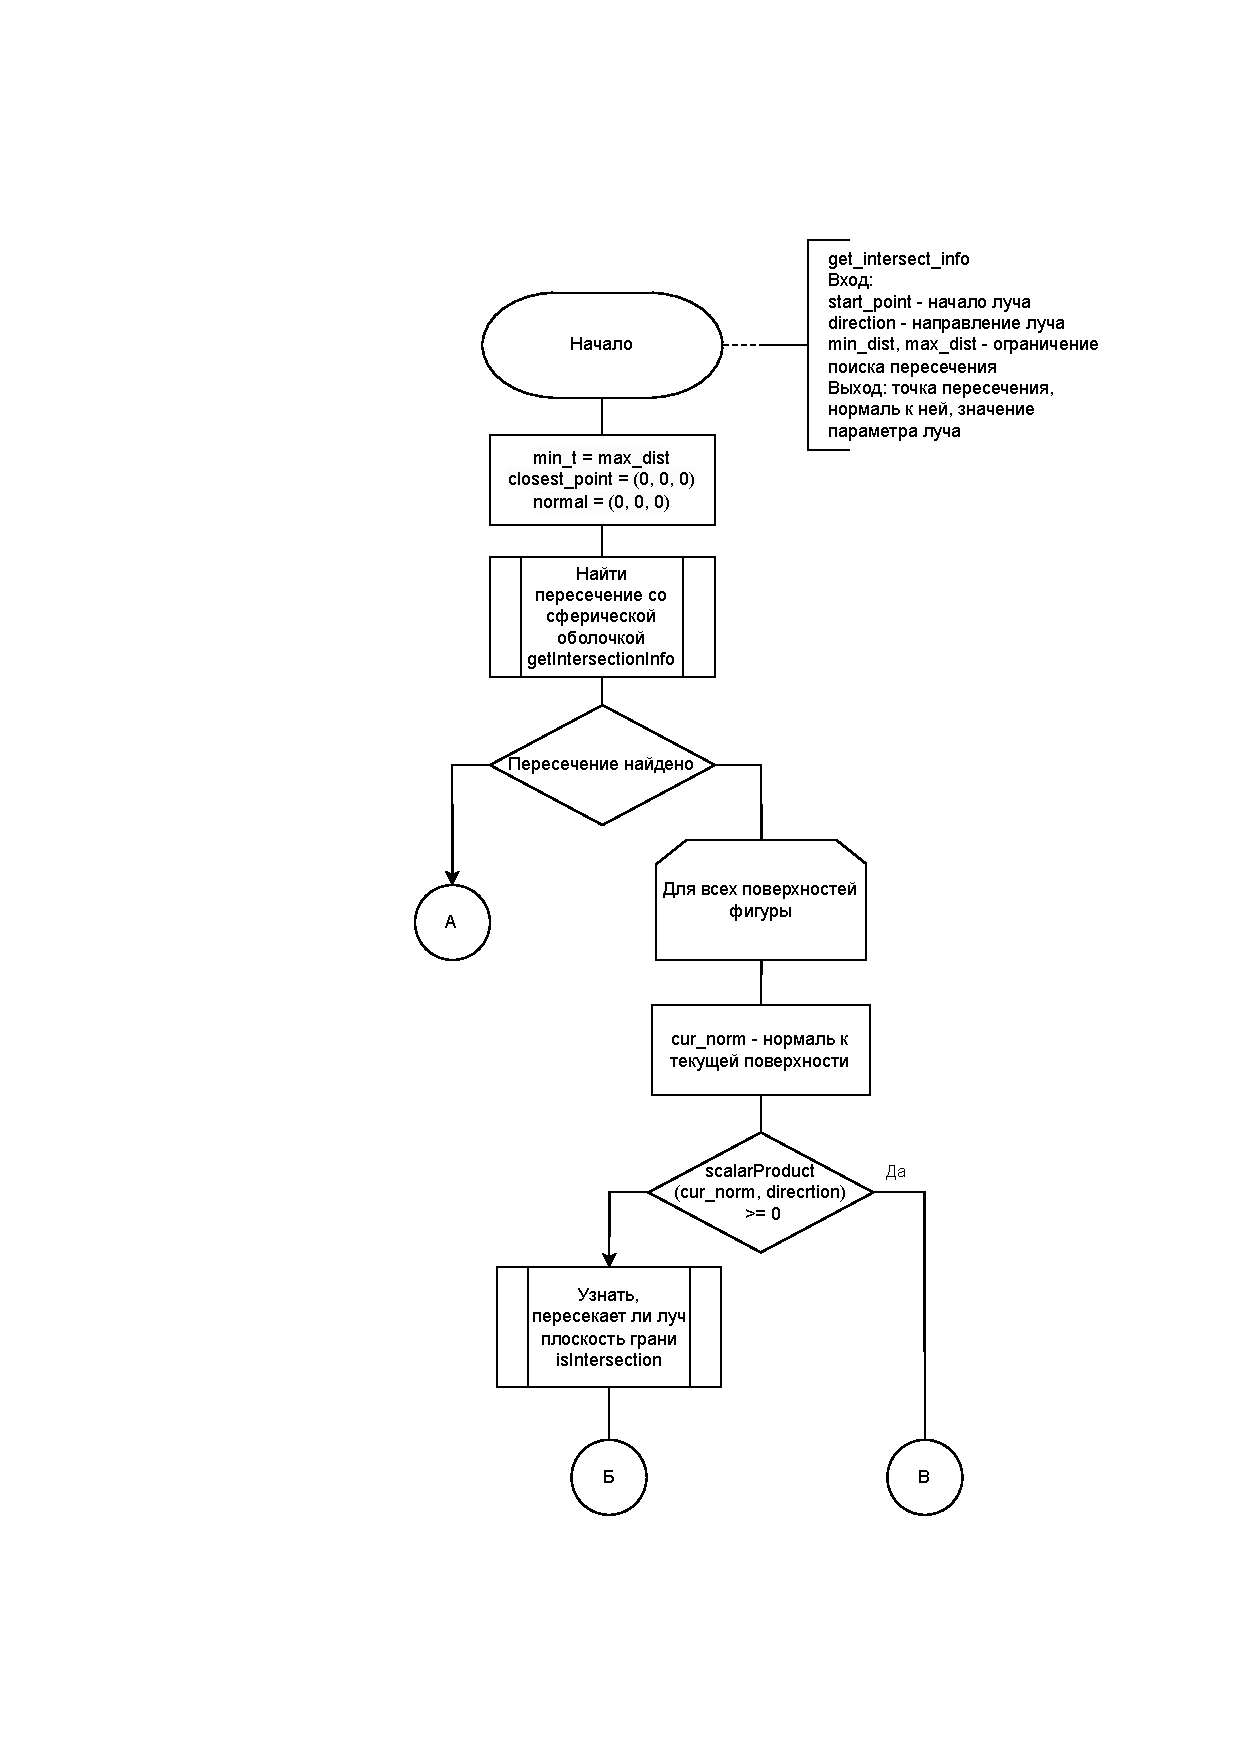
\includegraphics[width=\linewidth]{img/tr_intersection_1.pdf}
	\end{center}
	\captionsetup{justification=centering}
	\caption{Схема алгоритма поиска пересечения луча с триангулированным объектом (часть 1)}
	\label{img:tr_intersection_1}
\end{figure}

\begin{figure}[H]
	\begin{center}
		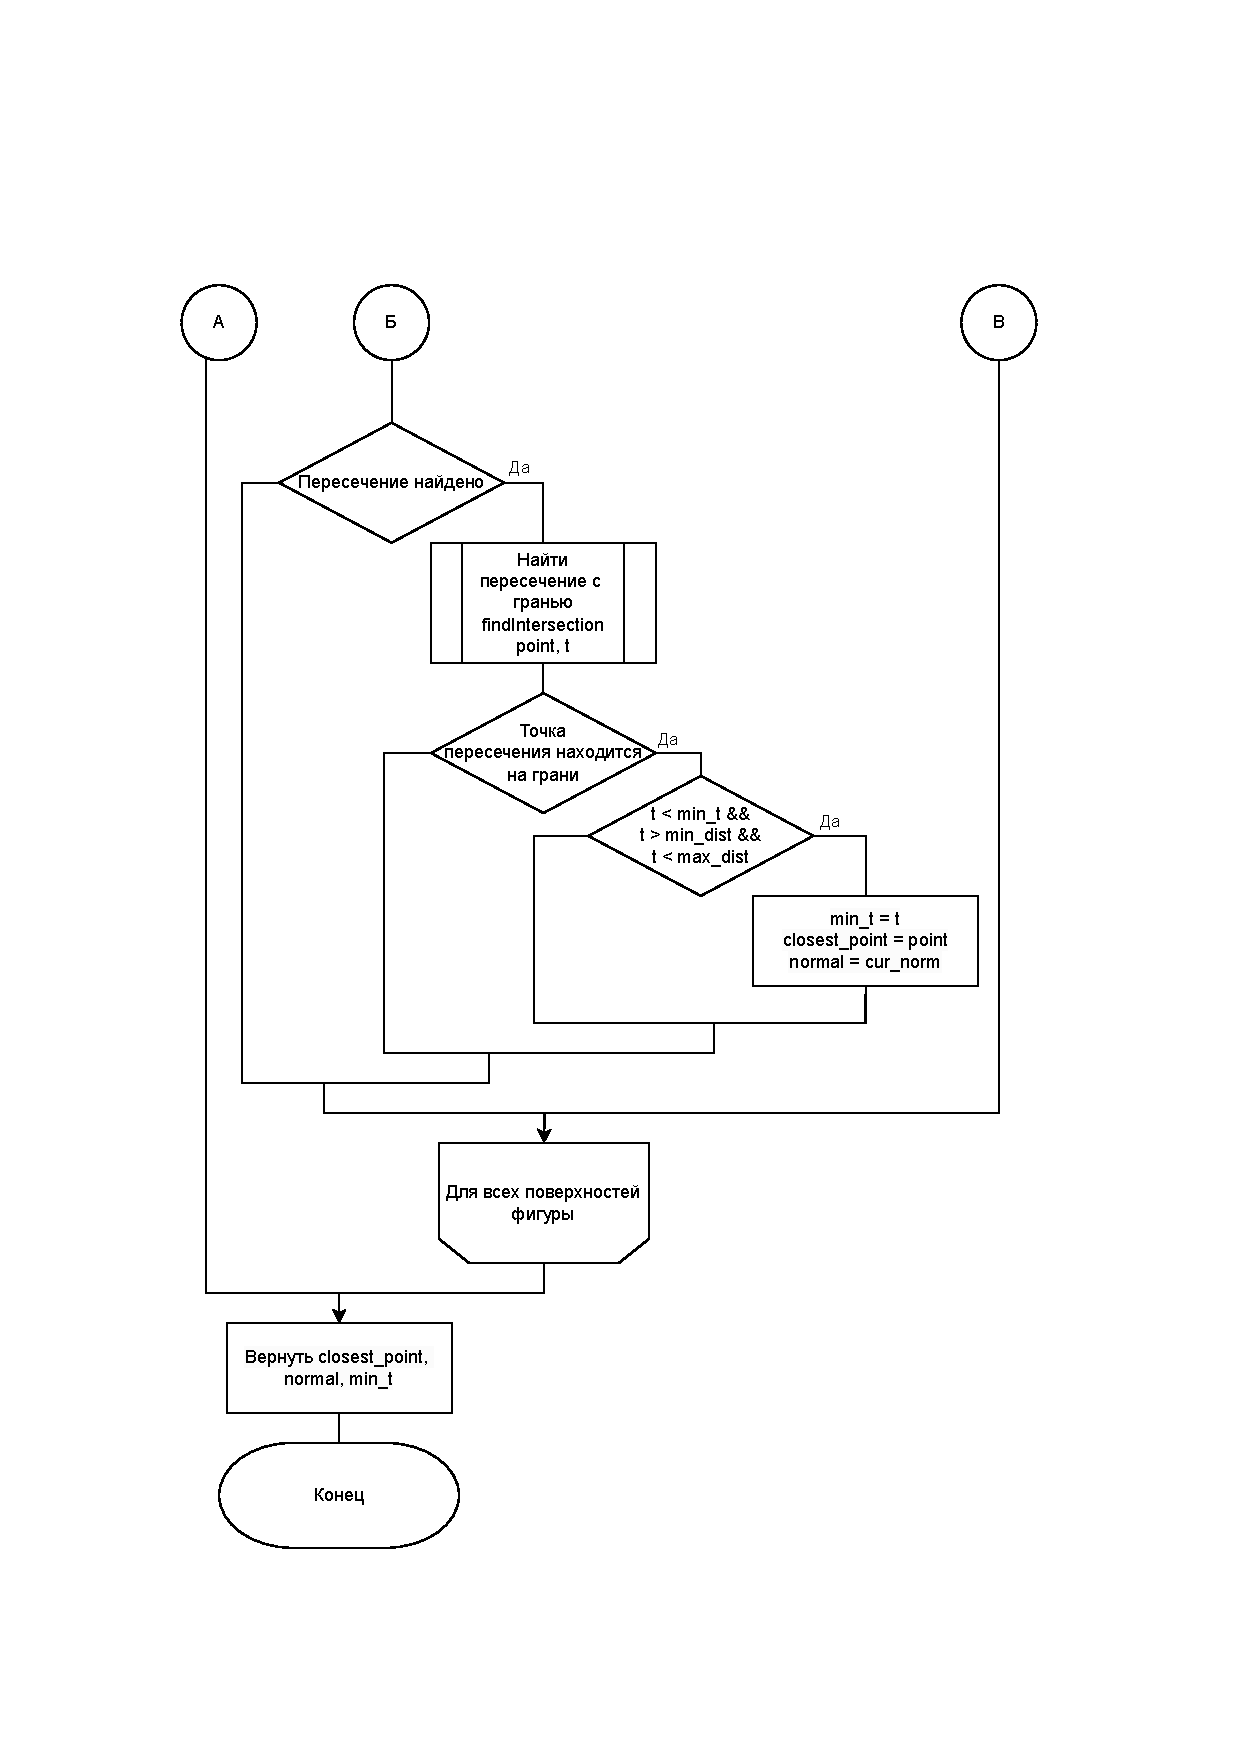
\includegraphics[width=\linewidth]{img/tr_intersection_2.pdf}
	\end{center}
	\captionsetup{justification=centering}
	\caption{Схема алгоритма поиска пересечения луча с триангулированным объектом (часть 2)}
	\label{img:tr_intersection_2}
\end{figure}

% =====================================================
\section{Математические основы алгоритмов}

Введём общие обозначения, используемые в формулах:

\begin{itemize}[label=---]
    \item $V$ -- точка, из которой трассируется луч;
    \item $D$ -- направление трассируемого луча.
\end{itemize}

Тогда трассируемый луч можно задать параметрическим уравнением:

\begin{equation}
P = V + tD
\end{equation}

Нас интересует только тот случай, когда $t > 0$, потому что тогда объект находится перед наблюдателем.

% -----------------------------------------------------
\subsection{Поиск пересечения луча со сферой}

Для поиска пересечения луча со сферой с центром в точке $C$ и радиусом $r$ необходимо решить следующую систему уравнений:

\begin{equation}
	\label{eq:sphere_intersect}
	\begin{cases}
		P = V + tD\\
		|P - C| = r\\
	\end{cases}
\end{equation}

Второе уравнение можно преобразовать следующим образом:

\begin{equation}
|P - C| = \sqrt{(P - C, P - C)}
\end{equation}

\begin{equation}
(P - C, P - C) = r^2
\end{equation}

Подставляем первое уравнение во второе:

\begin{equation}
t^2(D, D) + 2t(CO, D) + (CO, CO) - r^2 = 0
\end{equation}

 Введём следующие обозначения:

\begin{equation}
k_1 = (D, D),   k_2 = 2(OC, D),   k_3 = (CO, CO) - r^2
\end{equation}

\begin{equation}
k_1t^2 + k_2t + k_3 = 0
\end{equation}

Решениями данного квадратного уравнения являются значения параметра t, при которых луч пересекается со сферой:

\begin{equation}
\{ t_1, t_2 \} = {-k_2 \pm \sqrt{ {k_2}^2 -4k_1k_3} \over {2k_1}}
\end{equation}


% -----------------------------------------------------
\subsection{Поиск пересечения луча с триангулированным объектом}

Для поиска пересечения луча с триангулированным объектом, рассмотрим пересечение с его гранями.

Сначала необходимо проверить, пересекает ли луч плоскость, в которой лежит рассматриваемая грань (не пересекает только если параллелен).

\begin{equation}
(D, n) \neq 0
\end{equation}

Далее ищем пересечение с плоскостью грани, вершинами которой являются точки $A$, $B$ и $C$.

\begin{equation}
t = {(AV, n)\over(D, n)}
\end{equation}

Тогда точка пересечения $P$ будет равна:

\begin{equation}
P = V  + tD
\end{equation}

После этого проверяем, лежит ли точка пересечения в пределах грани. Для этого сводим задачу к 2х мерной, так как уже известно, что пересечение лежит в плоскости грани. Для этого координаты по оси OZ у вершин грани и точки пересечения обнуляем.

Далее считаем векторные произведения векторов стороны и векторов, соединяющих первую вершину с точкой пересечения.

\begin{equation}
v_1 = [AB, AP], v_2 = [BC, BP], v_3 = [CA, CP]
\end{equation}

Если все произведения имеют одинаковый знак, то точка лежит внутри грани.

Однако можно сразу отбросить ситуации, когда луч точно не пересечёт триангулированный объект. Для этого проверяется, пересекает ли луч сферу, описанную вокрг него. Тогда если луч не пересекает данную сферу, то он не может пересеч триангулированный объект.

Центр такой сферы совпадает с центром триангулированного объекта. А радиус совпадает с расстоянием от центра до наиболее удалённой от него точки.

% -----------------------------------------------------
\subsection{Поиск внешней нормали}

Внешней нормалью в точке $P$ сферы с центром в точке $C$ является вектор $CP$.

В триангулированном объекте каждая грань имеет свою нормаль. Найти нормаль грани можно следующим образом:

\begin{equation}
n = [BC, BA]
\end{equation}

Однако нормаль может оказаться внутренней, поэтому необходимо провести корректировку.

Нормаль является внешней если угол между ней и вектором проведённы от вершины к центру объекта тупой, это можно выразить следующим неравенством:

\begin{equation}
(BI, n) < 0
\end{equation}

Иначе необходимо домножить нормаль на $-1$.

% -----------------------------------------------------
\subsection{Поиск отражённого и преломлённого лучей}

Если вещество, из которого состоит объект, имеет ненулевой коэффициент зеркального отражения, трассируется луч, начинающийся в точке пересечения и имеющий направление отражённого луча относительно луча падения.

Если объект имеет ненулевой коэффициент пропускания, трассируется луч, начинающийся в точке пересечения и имеющий направление преломлённого луча относительно луча падения.

Луч падения, отражения, преломления и нормаль к поверхности лежат в одной плоскости. Луч падения и луч отражения имеют одинаковые углы с нормалью.

\begin{figure}[h]
	\centering
	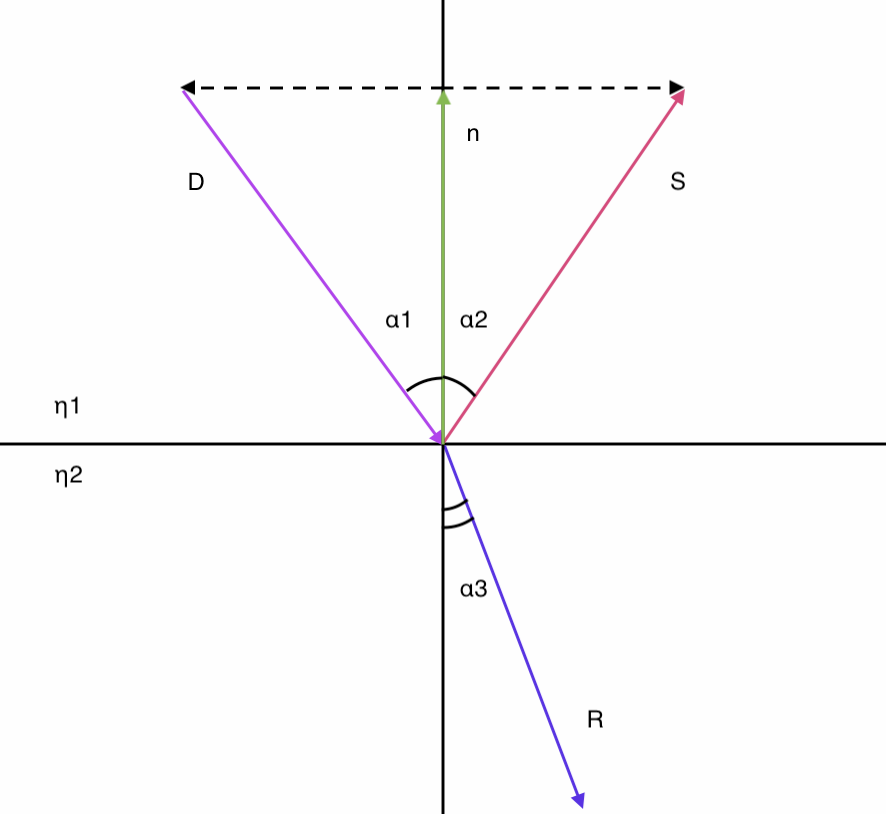
\includegraphics[width=0.5\textwidth]{img/specular_refract.png}
	\caption{Отражённый и преломлённый лучи}
	\label{fig:specular_refract}
\end{figure}

Отражённый луч находится следующим образом:

\begin{equation}
S = D - 2n(D, n).
\end{equation}

Пусть $\eta_i$ -- показатели преломления сред, причём $i = \overline{1,2}$. 
Применяя закон Снеллиуса, преломлённый луч можно найти следующим образом:

\begin{equation}
\begin{aligned}
R = \frac{\eta_1}{\eta_2}D + ( \frac{\eta_1}{\eta_2}\cos(\alpha_1) - \cos(\alpha_3))n, где
\end{aligned}
\end{equation}

\begin{equation}
\cos(\alpha_3) = \sqrt{1 - ({\eta_1\over\eta_2})^2(1 - \cos(\alpha_1))^2}.
\end{equation}

%=====================================================
\section{Выводы из конструкторской части}

В конструкторской части была представлена функциональная модель, спроектированно программное обеспечение для генерации изображения и представлены схемы алгоритмов.
